\documentclass{article}
\usepackage{underscore}
\usepackage{geometry}
\usepackage[utf8]{inputenc}
\usepackage{hyperref}
\usepackage{tikz}
\usetikzlibrary{shadows}
\usepackage{amsmath}  
\usepackage{booktabs}
\usepackage{newunicodechar}
\newunicodechar{ }{\,}
\newunicodechar{ }{\,}
\newunicodechar{≈}{\approx}
\newunicodechar{≈}{\approx}
\newunicodechar{∼}{\textasciitilde}
\newunicodechar{−}{\textminus}
\usepackage{booktabs}
\usepackage{pgfplotstable}
\pgfplotsset{compat=1.17}

\usetikzlibrary{positioning, shapes.geometric}

\usepackage{listings}
\lstset{breaklines=true, basicstyle=\ttfamily\small}

\title{How Cybersecurity Behaviors affect the Success of Darknet Drug Vendors: A Quantitative Analysis}
\author{\small Syon Balakrishnan and Aaron Grinberg}
\date{\small July 2025}

\begin{document}

\maketitle
\begin{abstract}
This study examines the relationship between cybersecurity behaviors and commercial success in darknet drug markets. Our analysis employs a large-scale dataset from the Agora marketplace, one of the largest drug-focused marketplaces operating between 2014 and 2015, to examine whether vendors mentioning Pretty Good Privacy (PGP) encryption capabilities achieve systematically different outcomes in terms of business scale, customer satisfaction, and competitive positioning. Our analytical approach nests encryption effects within a comprehensive framework that controls reputation accumulation, product diversification, pricing strategies, and category-specific market conditions, allowing us to isolate the unique contribution of cybersecurity signaling to commercial success while accounting for confounding behavioral and structural factors. Our findings illuminate several important mechanisms that shape competitive dynamics and vendor survival in anonymous digital commerce, with broader implications for policy, enforcement, and market regulation.
\end{abstract}
\section{Introduction and Literature Review}

The darknet represents an encrypted network on the Web that operates beyond the reach of conventional Internet infrastructure and law enforcement surveillance. These digital marketplaces have fundamentally transformed the landscape of illicit commerce, creating new channels for drug distribution that bypass traditional territorial controls and enforcement mechanisms. Drug sales represent a dominant use case in these markets, with recent estimates suggesting that global revenues exceed hundreds of millions of dollars annually~\cite{unodc2020}. Understanding the behavioral factors that drive vendor success in these anonymous environments has become critical to developing effective intervention strategies, as law enforcement agencies struggle to adapt their approaches to digital native criminal enterprises that leverage sophisticated cybersecurity practices to maintain operational security.

This study focuses specifically on how cybersecurity behaviors—particularly the signaling of encryption capabilities through Pretty Good Privacy (PGP) mentions—influence commercial success in darknet drug markets. Unlike conventional street-level drug markets, where vendor performance is shaped by social embeddedness, territorial enforcement, and face-to-face trust relationships, darknet markets mediate all interactions through pseudonymous profiles, customer reviews, and product listings. This fundamental shift from physical to digital commerce replaces direct interpersonal trust with digital reputation systems and behavioral signals, requiring vendors to develop entirely new forms of strategic behavior to establish credibility and attract customers in anonymous environments.

Four key dimensions emerge as theoretical drivers of vendor success in these digital marketplaces, each representing a different approach to building trust and competitive advantage without traditional business credentials or legal recourse mechanisms. Table~\ref{tab:mechanisms} outlines these four mechanisms—reputation signaling, product diversification, encryption use, and pricing strategy—that prior research has linked to vendor scale and longevity, forming the theoretical foundation for our empirical investigation.

\begin{table}[ht]
\centering
\begin{tabular}{|p{3.5cm}|p{4.5cm}|p{4.5cm}|}
\hline
\textbf{Mechanism} & \textbf{Rationale} & \textbf{Representative Literature} \\
\hline
Reputation Signaling & High ratings and feedback scores attract buyer trust and drive repeat transactions. & Christin (2013)~\cite{christin2013}, Janetos \& Tilly (2017)~\cite{janetos2017}, Eschenbaum \& Liebert (2021)~\cite{eschenbaum2021}, Andrei \& Veltri (2025)~\cite{andrei2025}, McBride (2023)~\cite{yelp2023} \\
\hline
Product Diversification & Vendors listing across multiple categories may reduce volatility and appeal to wider demand segments. & Crépino et al. (2019)~\cite{crepino2019}, Szigeti \& Molnár (2023)~\cite{szigeti2023}, Torre (2018)~\cite{torre2018}, Fonseca dos Reis et al. (2024)~\cite{fonseca2024multihomers}, Aitken et al. (2019)~\cite{aitken2019} \\
\hline
Encryption Signaling & PGP use may signal professionalism or reduce exposure to legal risk in vendor-buyer communication. & Dwyer et al. (2022)~\cite{dwyer2022}, UNODC (2020)~\cite{unodc2020}, Soska \& Christin (2015)~\cite{soska2015} \\
\hline
Price Strategy & Vendors may use competitive or prestige pricing to differentiate and influence buyer perceptions. & Aldridge \& Décary-Hétu (2016)~\cite{aldridge2016}, Zaunseder \& Koenig (2020)~\cite{zaunseder2020}, Barratt \& Aldridge (2016)~\cite{barratt2016} \\
\hline
\end{tabular}
\caption{Vendor Success Mechanisms in Darknet Markets and Supporting Literature}
\label{tab:mechanisms}
\end{table}

Reputation signaling constitutes the first critical dimension of vendor success, as customer feedback systems aggregated at the listing level serve as substitutes for in-person trust relationships in anonymous digital environments. Vendors must accumulate positive ratings and transaction volumes to demonstrate reliability, with higher-rated sellers attracting more traffic, commanding premium prices, and converting repeat customers more effectively. Past research consistently links high feedback scores to higher sales volumes, price premiums, and longer operational lifecycles, with some studies distinguishing between costly signals such as verified seniority and escrow usage versus superficial signals such as self-promotional descriptions~\cite{janetos2017, eschenbaum2021, andrei2025}. McBride~\cite{yelp2023} characterizes this reliance on digital reputation mechanisms as a form of "yelpification" of illicit commerce, where algorithmic feedback systems directly shape market outcomes and vendor survival.

Product diversification represents the second strategic dimension, as vendors who list products in multiple drug categories can hedge against demand uncertainty, maintain consistent listing presence during supply disruptions, and appeal to broader buyer segments seeking convenient one-stop-shop experiences. Torre~\cite{torre2018} frames this diversification as an intentional managerial strategy analogous to Ansoff's growth matrix, where vendors systematically expand product lines to stabilize revenues and reduce category-specific risks. The strategic importance of diversification becomes particularly evident when considering the inherent volatility of dark-net vendor participation. The useful lifetimes of darknet vendors are often remarkably short, with almost 45\% of Silk Road(anonymous black market for drugs and digital illicit trade) sellers remaining active for less than 30 days, although average tenures range between 90 and 100 days across different platforms~\cite{soska2015}. This high turnover rate underscores the precarious nature of vendor operations and highlights diversification as a potential survival mechanism, with blockchain-based network analyzes showing that multihoming strategies - a simultaneous presence in multiple marketplaces - support ecosystem resilience during market shutdowns and law enforcement actions~\cite{fonseca2024multihomers}.

Cybersecurity signaling and operational security practices constitute the third strategic dimension, where vendors advertise encryption capabilities and secure communication channels to signal both technical sophistication and commitment to protecting customer privacy. Secure communication through tools like PGP has become both a cultural and operational norm in darknet commerce, with vendors frequently posting public encryption keys in product listings to enable buyers to encrypt sensitive messages containing delivery addresses and payment information. Although such practices may provide genuine operational security benefits by reducing traceability and evidence generation, they also function as powerful professionalism signals within darknet communities where technical competence serves as a proxy for overall reliability and trustworthiness. Encryption technologies such as PGP create structural obstacles for law enforcement in dark-net drug markets, as these tools hinder monitoring, evidence collection, and intervention capabilities~\cite{unodc2020}. Within vendor communities, encryption functions simultaneously as both a normative expectation and a practical safeguard, and experienced sellers often advocate the use of PGP as a marker of professional competence~\cite{dwyer2022}. However, despite the widespread advocacy for encryption among experienced sellers documented in forum analyses~\cite{dwyer2022}, empirical research has yet to quantitatively link PGP usage patterns to actual commercial outcomes, representing a significant gap in our understanding of how cybersecurity behaviors translate into market success.

The pricing strategy constitutes the fourth theoretical dimension, as vendors can adopt various pricing approaches to differentiate their offerings and signal product quality or operational reliability. Vendors may employ competitive pricing to increase transaction volumes and market share, or alternatively adopt prestige pricing strategies that signal superior product quality or exclusive access to premium supplies. Zaunseder and Koenig~\cite{zaunseder2020} demonstrate that pricing decisions reflect complex interactions between vendor reputation, perceived product quality, and risk tolerance, while Soska and Christin~\cite{soska2015} document sophisticated pricing dynamics in which vendors temporarily pause listings to manage customer reviews and reset price expectations. Barratt and Aldridge~\cite{barratt2016} emphasize that high prices, when paired with detailed product descriptions and satisfaction guarantees, can serve as trust signals that communicate the vendor's confidence in product quality and service delivery. These pricing behaviors often coincide with other professional communication signals, such as encryption usage and escrow support, suggesting that successful vendors deploy integrated signaling strategies rather than relying on isolated tactics~\cite{vanhout2014, martin2014}. Vendor typologies ranging from corporate-style operations to boutique specialists can reflect differentiated pricing strategies that target distinct market segments with varying price sensitivity and quality expectations~\cite{munksgaard2016}.

\begin{table}[ht]
\scriptsize
\centering
\begin{tabular}{@{}p{4cm} p{7cm}@{}}
\toprule
\textbf{Study}                                     & \textbf{Primary Contribution}                                                    \\
\midrule
Christin (2013)~\cite{christin2013}               & Quantified Silk Road's economic footprint and vendor turnover.                 \\
Martin (2014)~\cite{martin2014}                   & Described trust-building and vendor motivations qualitatively.                 \\
Van Hout \& Bingham (2014)~\cite{vanhout2014}     & Explored harm-reduction and responsible vendor practices.                     \\
Munksgaard \& Demant (2016)~\cite{munksgaard2016} & Identified behavioral typologies among vendors.                                \\
Rhumorbarbe et al. (2016)~\cite{rhumorbarbe2016}  & Mapped geographical flows of online drug supply.                               \\
Décary-Hétu \& Giommoni (2017)~\cite{decary2017}  & Analyzed vendor strategies and sales predictors.                               \\
Duxbury \& Haynie (2020)~\cite{duxbury2020}       & Showed network centrality predicts vendor success.                            \\
Dwyer et al. (2022)~\cite{dwyer2022}               & Analyzed cybersecurity discourse and PGP norms.                               \\
UNODC (2020)~\cite{unodc2020}                      & Synthesized global trends and enforcement challenges.                         \\
\bottomrule
\end{tabular}
\caption{Research Focus and Contributions of Key Studies}
\label{tab:research-focus}
\end{table}

Despite this growing scholarly attention to darknet drug markets, few studies have systematically evaluated whether operational cybersecurity practices predict commercial success beyond their documented role in community norms and operational security. Existing research emphasizes reputation systems and pricing strategies as key performance drivers~\cite{christin2013, aldridge2016}, but cybersecurity signaling remains underexplored as a quantifiable behavioral predictor. Although qualitative studies have identified vendor professionalism typologies and marketing strategies~\cite{vanhout2014, munksgaard2016}, they rarely treat encryption practices as measurable factors that can be empirically linked to performance outcomes. This analytical gap limits our understanding of how vendors navigate the tension between operational security needs and commercial signaling requirements in technically sophisticated criminal environments.

The policy relevance of these research gaps has intensified as law enforcement capabilities continue to evolve beyond traditional market takedowns and arrest-based interventions. The United Nations Office on Drugs and Crime reports an increasing reliance on advanced digital forensics, cross-jurisdictional data sharing, and blockchain analytics to target the marketplace infrastructure and trace illicit financial flows~\cite{unodc2020}. However, vendor adoption of cybersecurity practices appears uneven across the ecosystem, with experienced sellers promoting encryption tools while many vendors omit basic security measures, reflecting heterogeneous levels of technical sophistication and risk awareness~\cite{dwyer2022}. Understanding whether cybersecurity signaling correlates with commercial success could inform both enforcement targeting strategies and harm reduction approaches that seek to influence vendor behavior through market dynamics.

Figure~\ref{fig:venn} illustrates the conceptual domains that underpin vendor success and positions our study's focus on encryption signaling within the broader theoretical landscape.

\begin{figure}[ht]
\centering
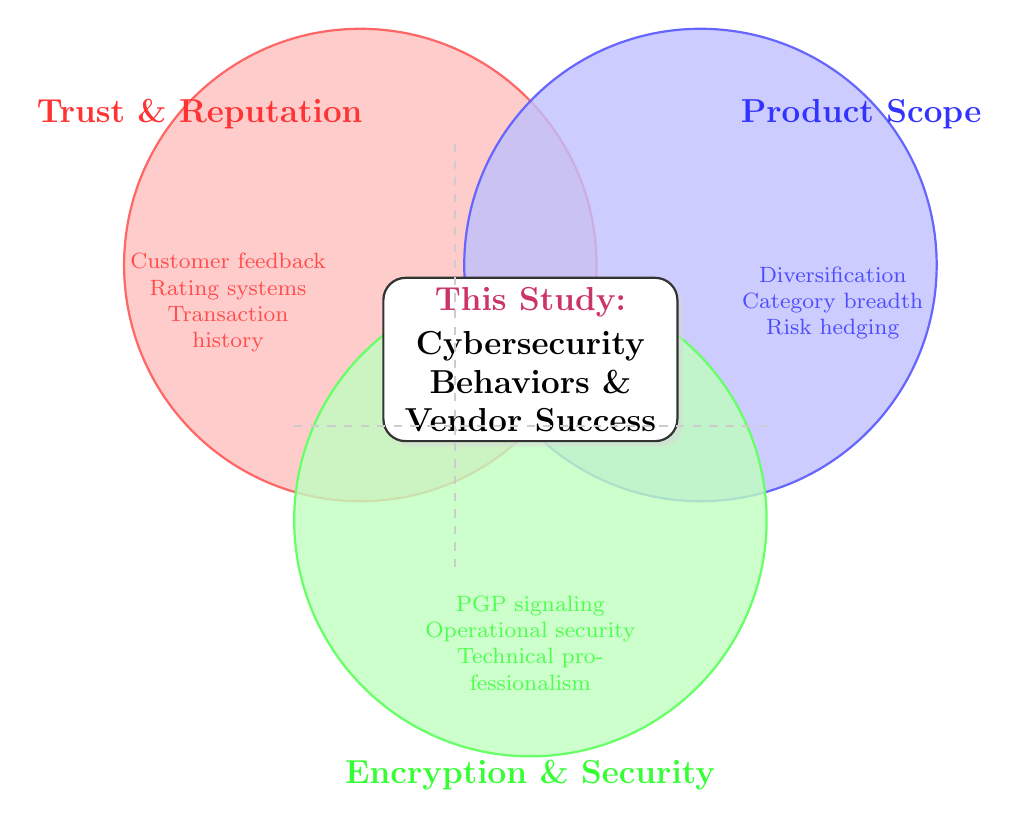
\begin{tikzpicture}[scale=1.2]
  % Circle 1 - Trust/Reputation (top left)
  \begin{scope}
    \fill[red!25, opacity=0.8] (-0.8,1.2) circle (2.5cm);
    \draw[red!60, thick] (-0.8,1.2) circle (2.5cm);
    \node[font=\large\bfseries, text=red!80] at (-2.5,2.8) {\textsc{Trust \& Reputation}};
    \node[font=\footnotesize, text=red!70, text width=2.5cm, align=center] at (-2.2,0.8) {Customer feedback\\Rating systems\\Transaction history};
  \end{scope}
  
  % Circle 2 - Product Scope (top right)  
  \begin{scope}
    \fill[blue!25, opacity=0.8] (2.8,1.2) circle (2.5cm);
    \draw[blue!60, thick] (2.8,1.2) circle (2.5cm);
    \node[font=\large\bfseries, text=blue!80] at (4.5,2.8) {\textsc{Product Scope}};
    \node[font=\footnotesize, text=blue!70, text width=2.5cm, align=center] at (4.2,0.8) {Diversification\\Category breadth\\Risk hedging};
  \end{scope}
  
  % Circle 3 - Encryption/Cybersecurity (bottom)
  \begin{scope}
    \fill[green!25, opacity=0.8] (1,-1.5) circle (2.5cm);
    \draw[green!60, thick] (1,-1.5) circle (2.5cm);
    \node[font=\large\bfseries, text=green!80] at (1,-4.2) {\textsc{Encryption \& Security}};
    \node[font=\footnotesize, text=green!70, text width=3cm, align=center] at (1,-2.8) {PGP signaling\\Operational security\\Technical professionalism};
  \end{scope}
  
  % Central study focus box
  \node[rectangle, fill=white, draw=black!80, thick, rounded corners=8pt, 
        text width=3.5cm, align=center, font=\large\bfseries,
        drop shadow={shadow xshift=2pt, shadow yshift=-2pt, fill=gray!30}] 
        at (1,0.2) {
        \textcolor{purple!80}{\textsc{This Study:}}\\[2pt]
        \textcolor{black}{Cybersecurity}\\
        \textcolor{black}{Behaviors \&}\\
        \textcolor{black}{Vendor Success}
        };
        
  % Add some decorative elements
  \draw[gray!40, dashed, thick] (-1.5,-0.5) -- (3.5,-0.5);
  \draw[gray!40, dashed, thick] (0.2,-2) -- (0.2,2.5);
  
\end{tikzpicture}
\caption{Conceptual framework: theoretical domains underpinning vendor success in darknet markets and this study's focus on cybersecurity signaling.}
\label{fig:venn}
\end{figure}

This study addresses these theoretical and policy gaps by providing the first large-scale regression-based analysis of encryption signaling effects on vendor performance outcomes. Using data from over 2,600 vendors operating in the Agora marketplace between 2014 and 2015, we examine whether vendors mentioning PGP encryption capabilities achieve systematically different outcomes in terms of business scale, customer satisfaction, and competitive positioning. Our analytical approach nests encryption effects within a comprehensive framework that controls reputation accumulation, product diversification, pricing strategies, and category-specific market conditions, allowing us to isolate the unique contribution of cybersecurity signaling to commercial success while accounting for confounding behavioral and structural factors.

Previous research has consistently shown that reputation systems and product diversification are important predictors of vendor visibility and operational resilience in darknet markets. However, cybersecurity practices, particularly encryption signaling, remain largely unexamined as quantifiable behavioral drivers of commercial performance. Although studies have documented widespread PGP advocacy in vendor communities and identified encryption as a cultural norm, empirical evidence linking these practices to measurable business outcomes remains scarce. Our analysis bridges this gap by testing whether vendors that signal encryption capabilities are systematically more successful across multiple performance dimensions, examining this relationship alongside established theoretical drivers, including reputation accumulation, diversification strategies, and pricing approaches. This comprehensive modeling framework allows us to determine whether cybersecurity signaling represents an independent pathway to commercial success or simply correlates with other vendor characteristics that drive market performance in anonymous digital environments.
\section{Methods}
\label{sec:methods}

Our analysis employs a comprehensive quantitative framework to examine the relationship between cybersecurity behaviors and vendor success in dark-net drug markets. We utilized a large-scale dataset from the Agora marketplace, implementing sophisticated variable construction techniques and nested regression modeling to isolate causal mechanisms.

\subsection{Data Sources and Sample Construction}

Our analysis is based on a structured data set of over 100,000 unique darknet listings from Agora, one of the largest drug-focused marketplaces operating between 2014 and 2015. The raw data originate from an HTML scrape posted by a Reddit user known as "usheep," who extracted the listings from Agora's surface-web front-end and later publicly released the archive. A Kaggle user, \texttt{philipjames11}, subsequently cleaned and structured this data set into tabular format, removing duplicates and averaging prices for listings that appeared multiple times.

The resulting dataset contains detailed metadata for each listing, including the seller's pseudonymous vendor name, hierarchical product classification, item titles, free-text descriptions containing operational details, averaged Bitcoin prices, geographic shipping claims, textual customer feedback ratings, and notes on potential pricing outliers. The hierarchical category structure follows the pattern \texttt{Drugs/Cannabis/Weed}, enabling both primary and secondary classification analysis.

Our sampling procedure implements multiple quality control filters to ensure analytical rigor. We first restrict the sample to listings with standardized Bitcoin pricing and numerical ratings matching the pattern \verb!^\d+\.\d+/5$! to ensure homogeneous measurement units. We then limit our analysis to drug and tobacco related categories to maintain a focus on illicit substance markets. This filtering process yields approximately 50,000 listings from 2,653 unique vendors, forming our analytical sample.\footnote{\url{https://github.com/syoncodes/agora-regression}}

\subsection{Variable Construction and Feature Engineering}

\subsubsection{Dependent Variables}

We construct vendor-level measures by aggregating listing-level data across four key dimensions of marketplace success. Our primary scale indicator, \texttt{total_listings}, represents the raw count of unique product listings per vendor, serving as our main measure of business scope without transformation to allow for intuitive interpretation of coefficients. The product diversification measure, \texttt{number_categories}, counts the number of distinct drug categories in which each vendor operates, capturing strategic diversification decisions that can provide insurance against demand volatility and enforcement targeting.

Financial performance is captured through \texttt{avg_price_btc}, which represents the mean Bitcoin price across all listings for each vendor, reflecting the pricing strategy and product positioning. This variable exhibits substantial right-skew due to high-value bulk transactions and premium products. Quality assessment is measured through \texttt{avg_rating}, which aggregates customer feedback scores on a scale of 1-5, providing information on buyer satisfaction and perceived service quality. The compressed distribution of this variable, with a mean of 4.83 and a median of 4.98, reflects either selection effects or reporting biases common in anonymous marketplaces.

\subsubsection{Primary Predictor Variables}

Our key predictor variable, \texttt{pgp\_present}, employs case-insensitive string matching to identify vendors who mention Pretty Good Privacy (PGP) encryption in any listing description. This binary indicator captures vendors who signal cryptographic capability regardless of the frequency of mention, reflecting our theoretical focus on signaling rather than operational security implementation. The detection algorithm searches for the exact string "PGP" within product descriptions, flagging any vendor with at least one mention throughout their entire product portfolio.

The product diversification strategy is quantified through \texttt{ number_categories}, which measures the breadth of each vendor's product portfolio across our ten-category drug taxonomy. These categories include Cannabis, Dissociatives, Ecstasy, Opioids, Prescription, Psychedelics, RCs (Research Chemicals), Steroids, Stimulants, OtherMinor. This measure captures strategic diversification decisions that can serve as insurance against category-specific enforcement actions or demand fluctuations.

Professional signaling is assessed through a comprehensive classifier that measures the proportion of each vendor's listings containing professional terminology. The \texttt{pct\_professional} variable is calculated as the percentage of listings that contain any term from our curated professional vocabulary:

\begin{equation}
\text{pct\_professional}_j = \frac{1}{N_j} \sum_{i=1}^{N_j} \mathbf{1}[\text{professional\_terms} \in \text{description}_{ij}]
\end{equation}

where $N_j$ represents the total listings for vendor $j$, and the indicator function flags the descriptions that contain any term from our professional set.

Our set of professionalism terms includes twenty carefully selected indicators that span multiple dimensions of vendor sophistication. Operational security terms include stealth, vacuum sealed, vacuum sealed, discreet, and sealed. Quality assurance indicators encompass lab-tested, lab-tested, purity, pharmaceutical name, and blister pack. Customer service signals comprise tracking, tracking number, refund, guarantee, reship, and business days. Technical proficiency is marked by terms such as escrow and public key, while community engagement is indicated by read profile and erowid references.

We explicitly exclude common but noninformative terms such as "tablet," "pack" and "bottle" that appear frequently but do not signal professional practices. This approach captures multiple dimensions of vendor professionalism, including operational security, quality control, customer service excellence, and community engagement.

\subsubsection{Drug Category Classification System}

We implement a dual-level classification system that captures both primary specialization and secondary diversification patterns throughout our drug taxonomy. Primary categories are extracted from the main hierarchical category field, while secondary categories are derived from the second-level classification token. For example, a list categorized as "Drugs/Cannabis/Weed" would have Cannabis as its secondary classification token. This dual classification approach allows us to distinguish between vendors that specialize primarily in specific drug types and those who offer them as secondary products within diversified portfolios.

For each of our ten drug categories, we create both primary and secondary binary indicators. Primary indicators flag vendors who have any listing in a particular category, while secondary indicators are derived from the hierarchical structure's second level. This system enables nuanced analysis of category-specific effects while controlling for diversification patterns and allows us to capture different levels of specialization and market positioning strategies.

\subsubsection{Success Outcome Definitions}

We define three binary success indicators to capture different dimensions of vendor performance in the marketplace hierarchy. Elite performance, measured by \texttt{ top_vendor}, identifies vendors in the top decile by listing volume, representing approximately 265 vendors who achieve truly exceptional scale. The above average performance, captured by the large vendor \texttt{}, includes vendors that exceed the median listing count, representing the upper half of the scale distribution. Quality excellence, measured through \texttt{ high_rating}, identifies vendors who achieve above-median average ratings, indicating superior customer satisfaction despite the compressed nature of the rating distribution.

These indicators allow us to examine whether encryption signaling and other behaviors predict different types of marketplace success, from achieving basic viability to reaching elite status. The multidimensional approach recognizes that success in anonymous markets may manifest differently in scale, profitability, and quality dimensions.

\subsection{Statistical Modeling Strategy}

\subsubsection{Nested Regression Framework}

We employ a nested regression approach that introduces predictor blocks sequentially to isolate the marginal contribution of each theoretical mechanism. This methodology is crucial for understanding whether PGP signaling represents an independent causal factor or serves as a proxy for other vendor characteristics that drive success in anonymous digital markets.

Our five-block structure systematically controls for alternative explanations while preserving the ability to observe how coefficient estimates change as additional mechanisms are introduced. The first block establishes the bivariate association between PGP presence and outcomes, providing the baseline relationship without controls. The second block adds product diversification through \texttt{num\_categories}, testing whether apparent encryption effects are driven by underlying diversification strategies that may be correlated with professional signaling.

The third block incorporates average pricing through \texttt{avg_price_btc} to control for product positioning and market segment effects that could confound the relationship between signaling behaviors and success outcomes. The fourth block adds the percentage of professional signaling through \texttt{ pct_professional} to test whether PGP mentions are simply part of broader professionalism strategies rather than independent predictors of success. The final block includes comprehensive drug class controls, incorporating both primary and secondary category indicators to account for systematic differences in market conditions, enforcement intensity, and operational constraints across substance types.

This progressive specification allows us to observe how the estimated PGP effect evolves as alternative mechanisms are controlled for, providing crucial insights into the causal structure underlying vendor success patterns. If PGP effects attenuate substantially when other factors are controlled, this suggests the encryption signaling may be serving as a proxy for unobserved vendor characteristics rather than representing an independent causal mechanism.

\subsubsection{Model Specifications and Estimation}

For vendor scale measured by \texttt{ total_listings} and rating quality measured by \texttt{avg_rating}, we estimate ordinary least-squares models using raw counts rather than logarithmic transformations. This specification choice facilitates an intuitive interpretation of coefficients as expected changes in listing counts or rating points associated with each predictor. We employ HC3 robust standard errors to address heteroskedasticity arising from substantial variation in vendor scales and business models observed in the data.

For binary success outcomes including \texttt{top\_vendor}, \texttt{large\_vendor}, and \texttt{high\_rating}, we estimate logistic regression models. The logistic specification models the probability of success as follows:

\begin{equation}
\Pr(Y_j = 1|\mathbf{X}_j) = \frac{\exp(\alpha + \mathbf{X}_j\boldsymbol{\beta})}{1 + \exp(\alpha + \mathbf{X}_j\boldsymbol{\beta})}
\end{equation}

where $Y_j$ represents the binary outcome for the vendor $j$, $\mathbf{X}_j$ is the predictor vector, and $\boldsymbol{\beta}$ contains the coefficients of interest. We report odds ratios for intuitive interpretation, representing the multiplicative change in odds associated with each predictor.

When computationally feasible, we employ robust HC3 standard errors for logistic models to maintain consistency with our linear specifications. In cases where convergence issues arise with robust estimation, we fall back to default standard errors while noting this limitation in our results presentation.

\subsubsection{Model Selection and Robustness}

We compare our primary OLS specification against Poisson generalized linear models to account for the count nature of the listing outcome variable. Model selection is based on the Akaike Information Criterion (AIC) and Bayesian Information Criterion (BIC), with preference given to specifications that demonstrate superior fit while maintaining interpretability. Our analysis reveals that OLS models achieve superior performance on both criteria and exhibit acceptable residual diagnostics, which leads us to retain OLS as our primary specification.

Comprehensive residual diagnostics include examination of Q-Q plots for normality assessment and residual versus fitted value plots for heteroscedasticity detection. We identify influential observations using standard diagnostic measures and perform sensitivity analyzes to ensure that our results are not driven by outliers or unusual vendor characteristics.

Fixated effects of the drug class capture category-specific factors that can influence the scale or success of the vendor regardless of the strategies of the individual vendor. These controls are particularly important given the differential enforcement attention and operational constraints between different types of substances. The inclusion of both primary and secondary category indicators allows for nuanced control of specialization patterns while maintaining statistical power for our main effects of interest.

All models are estimated using Python 3.9 with the statsmodels library, ensuring reproducible results and robust numerical optimization. Convergence criteria are set to standard tolerances, with alternative optimization algorithms employed when necessary to ensure stable parameter estimates across all model specifications.

\subsubsection{Model Selection and Diagnostic Assessment}

We compare our primary OLS specification against Poisson generalized linear models to account for the count nature of the listing outcome variable. Table~\ref{tab:robust_models} presents the results of the model comparison based on information criteria.

\begin{table}[ht]
  \centering
  \begin{tabular}{lcc}
    \toprule
    Model & AIC & BIC\\
    \midrule
    OLS (raw counts, HC3 SEs) & 27\,387 & 27\,475\\
    Poisson (raw count)       & 84\,623 & 51\,389\\
    \bottomrule
  \end{tabular}
  \caption{Comparison of OLS (raw counts) and Poisson models}
  \label{tab:robust_models}
\end{table}

The OLS specification demonstrates a superior fit based on model diagnostics and interpretability considerations. Our primary OLS model (Model 5) achieves an AIC of 27,387, with acceptable residual diagnostics, as shown in the diagnostic plots below. This substantial difference in model fit, combined with the interpretability advantages of OLS coefficients, leads us to retain ordinary least squares as our primary specification.

\paragraph{Residual Diagnostics.} Figure~\ref{fig:qq_logols} presents the Q-Q plot of Pearson residuals from our primary OLS specification, demonstrating acceptable adherence to normality assumptions despite some deviation in the extreme tails. This pattern is consistent with the count nature of our outcome variable and the presence of high-volume outlier vendors in our sample.

\begin{figure}[ht]
  \centering
  \includegraphics[width=.6\textwidth]{qq_plot_rawols.pdf}
  \caption{Q–Q plot of Pearson residuals from the OLS (raw counts) model.}
  \label{fig:qq_logols}
\end{figure}

Figure~\ref{fig:resid_fitted} shows the relationship between the raw residuals and the fitted values, revealing some heteroskedasticity that justifies our use of robust standard errors of HC3. The residual pattern shows an increase in variance at higher fitted values, reflecting the greater variability in business models among large-scale vendors compared to smaller operators.

\begin{figure}[ht]
  \centering
  \includegraphics[width=.6\textwidth]{resid_vs_fitted_rawols.pdf}
  \caption{Raw residuals vs.\ fitted values for the OLS (raw counts) model.}
  \label{fig:resid_fitted}
\end{figure}

These diagnostic plots confirm that while perfect normality and homoscedasticity are not achieved, the deviations are manageable through robust standard error correction and do not substantially compromise the validity of our statistical inferences.

\section*{Appendix A: Complete Professionalism Term List}

The following terms were used to identify professional practices in vendor listings (case-insensitive matching):

blister pack, business days, discreet, erowid, escrow, guarantee, lab-tested, lab-tested, pharmaceutical name, public key, purity, read profile, refund, reship, sealed, stealth, tracking, tracking number, vacuum sealed, vacuum-sealed.

Terms explicitly excluded from the professionalism classifier: "tablet," "pack," "bottle."

\section{Results}\label{sec:results}

\begin{table}[htbp]
  \centering
  \scriptsize
  \setlength\tabcolsep{4pt}
  \begin{tabular}{lrrrrr}
    \toprule
    Variable              &   Mean & Median &    SD &    Min &      Max \\
    \midrule
    total\_listings       &  32.68 & 18.00 & 49.25 &  1.00 &  815.00 \\
    num\_categories       &   3.33 &  2.00 &  2.80 &  1.00 &   24.00 \\
    avg\_price\_btc       &  16.88 &  0.77 &260.10 &  0.00 &10892.16 \\
    avg\_rating           &   4.83 &  4.98 &  0.55 &  0.00 &    5.00 \\
    \bottomrule
  \end{tabular}
  \caption{Descriptive statistics ($N=2\,653$ vendors).}
  \label{tab:descriptives}
\end{table}

Our analysis includes 2,653 unique vendors operating in the Agora marketplace. Table~\ref{tab:descriptives} reveals substantial heterogeneity in vendor characteristics and business strategies. The typical vendor maintains a moderate-scale operation with 18 listings (median), though the mean of 32.7 listings suggests a right-skewed distribution driven by high-volume sellers. In fact, the most prolific vendor advertised 815 different products, representing a scale of operations 45 times larger than the median seller. This distribution reflects the ``long tail'' structure common to digital marketplaces, where a small number of large vendors coexist with many smaller operators.

Product diversification patterns show similar variation. Although the median vendor operates in only two drug categories, the mean of 3.3 categories indicates that many sellers pursue broader product portfolios. The most diversified vendor spanned 24 different categories, suggesting highly sophisticated operations that may require substantial inventory management and supplier relationships across multiple drug types.

Pricing exhibits extreme heterogeneity, with Bitcoin values ranging from fractions of a coin to more than 10,892 BTC. The median price of 0.77 BTC contrasts sharply with the mean of 16.88 BTC, indicating that high-value transactions, which are likely bulk sales or expensive drugs such as high-grade stimulants or research chemicals, substantially influence the overall price distribution. This variance reflects both the diversity of products offered and the range of transaction sizes, from small retail purchases to wholesale-level deals.

Customer satisfaction metrics cluster near the ceiling, with ratings averaging 4.83 out of 5 and a median of 4.98. The narrow standard deviation of 0.55 suggests that most vendors achieve relatively high customer satisfaction, though the minimum rating of 0 indicates that some vendors do not meet buyer expectations. This compressed distribution may reflect selection effects: poorly rated vendors may exit the market quickly—or buyer reluctance to post negative reviews in anonymous environments.

\subsection{Vendor Scale Analysis}

Figure~\ref{fig:box_pgp} compares the raw distribution of listings between vendors who mention PGP encryption and those who do not. The violin plot reveals that PGP advertising vendors consistently operate at larger scales across the distribution. Most strikingly, the median PGP vendor maintains approximately twice as many listings as the median non-PGP vendor, suggesting a strong bivariate association between encryption signaling and business scale.

\begin{figure}[htbp]
  \centering
  \includegraphics[width=.75\textwidth]{violin_pgp_size.pdf}
  \caption{Distribution of total listings (log scale) by PGP mention.}
  \label{fig:box_pgp}
\end{figure}

To isolate the causal mechanisms underlying this relationship, we estimated a series of nested OLS models that progressively add controls for alternative explanations. Table~\ref{tab:ols_size_nested} documents how the estimated effects of PGP encryption signaling and product diversification evolve as additional covariates are introduced.

\begin{table}[htbp]
  \centering
  \scriptsize
  \setlength\tabcolsep{4pt}
  \begin{tabular}{lrrrrrr}
    \toprule
    & \multicolumn{3}{c}{\textbf{PGP Present}} & \multicolumn{3}{c}{\textbf{Number of Categories}} \\
    \cmidrule(lr){2-4} \cmidrule(lr){5-7}
    Model & Coef. & SE & Sig. & Coef. & SE & Sig. \\
    \midrule
    1 & 11.578 & 4.200 & *** & — & — & — \\
    2 &  4.927 & 4.022 &  & 8.674 & 0.775 & *** \\
    3 &  4.984 & 4.022 &  & 8.675 & 0.776 & *** \\
    4 &  4.931 & 4.065 &  & 8.673 & 0.772 & *** \\
    5 &  5.608 & 4.040 &  & 11.810 & 1.573 & *** \\
    \bottomrule
  \end{tabular}
  \caption{Nested OLS models predicting total listings. Model 1: PGP only; Model 2: + Categories; Model 3: + Price; Model 4: + Professionalism; Model 5: + Drug class fixed effects. Stars: $^{***}p<0.01$, $^{**}p<0.05$, $^{*}p<0.1$.}
  \label{tab:ols_size_nested}
\end{table}

The progression reveals a striking pattern. In the bivariate specification (Model 1), PGP presence predicts an additional 11.58 listings on average—a substantial effect representing a 35\% increase over the sample mean. This coefficient is highly significant ($p < .01$), initially suggesting that encryption signaling may be a powerful predictor of vendor success. However, this interpretation changes dramatically once product diversification enters the model.

The inclusion of \texttt{num\_categories} in Model 2 reduces the PGP coefficient to 4.93 listings and renders it statistically insignificant. This effect remains stable across Models 2-5 as price controls, professionalism measures, and drug-class fixed effects are added, with the final PGP coefficient settling at 5.61 listings ($p = .165$). In contrast, the diversification effect strengthens as controls are added, reaching 11.81 additional listings per category in the full specification ($p < .001$).

This pattern suggests that the apparent association between PGP and vendor scale is largely spurious, driven by the correlation between encryption signaling and product diversification. Vendors who operate across multiple drug categories may be more likely to advertise encryption capabilities as part of a broader professionalism strategy, but it is the diversification itself—not the encryption signaling—that drives business scale.

The full model results (Table~\ref{tab:ols_size_full}) provide additional insights into the factors that constrain or enable vendor growth.

\begin{table}[htbp]
  \centering
  \scriptsize
  \setlength\tabcolsep{4pt}
  \begin{tabular}{lrrrrr}
    \toprule
    & \multicolumn{5}{c}{\textbf{DV: Total listings}}\\
    \cmidrule(lr){2-6}
    Variable & M1 & M2 & M3 & M4 & M5\\
    \midrule
    Intercept               & 32.076*** & 3.531     & 3.443     & -17.610*** & -14.730***\\
    PGP present             & 11.578**  & 4.927     & 4.984     & 4.676      & 5.389\\
    \# Categories           &           & 8.674***  & 8.675***  & 8.645***   & 11.810***\\
    Avg.\ Price (BTC)       &           &           & 0.005     & 0.005      & 0.005\\
    Pct.\ Professional      &           &           &           & 0.931      & 2.827\\
    Avg.\ Rating            &           &           &           & 4.342***   & 4.106***\\
    \addlinespace
    \multicolumn{6}{l}{\emph{Primary drug class}}\\
    Cannabis                &           &           &           &            & 0.714\\
    Dissociatives           &           &           &           &            & -3.300*\\
    Ecstasy                 &           &           &           &            & -2.377*\\
    Opioids                 &           &           &           &            & -8.051***\\
    Other Minor             &           &           &           &            & 0.000\\
    Prescription            &           &           &           &            & -3.803\\
    Psychedelics            &           &           &           &            & -3.899***\\
    RCs                     &           &           &           &            & -1.150\\
    Steroids                &           &           &           &            & 2.537\\
    Stimulants              &           &           &           &            & -3.834**\\
    \addlinespace
    \multicolumn{6}{l}{\emph{Secondary drug class}}\\
    Cannabis (sec)          &           &           &           &            & 0.714\\
    Dissociatives (sec)     &           &           &           &            & -3.300*\\
    Ecstasy (sec)           &           &           &           &            & -2.377*\\
    Opioids (sec)           &           &           &           &            & -8.051***\\
    Other Minor (sec)       &           &           &           &            & 0.000\\
    Prescription (sec)      &           &           &           &            & -6.402\\
    Psychedelics (sec)      &           &           &           &            & -3.899***\\
    RCs (sec)               &           &           &           &            & -1.150\\
    Steroids (sec)          &           &           &           &            & 2.537\\
    Stimulants (sec)        &           &           &           &            & -3.834**\\
    \midrule
    \multicolumn{6}{l}{\footnotesize Stars: $^{*}p<0.05$, $^{**}p<0.01$, $^{***}p<0.001$. Robust SE: HC3.}\\
    \bottomrule
  \end{tabular}
  \caption{Nested OLS predicting total listings (Models 1–5).}
  \label{tab:ols_size_nested}
\end{table}

Several drug classes show significant negative associations with vendor scale relative to the baseline category. Opioid vendors face particularly severe constraints, averaging 8.05 fewer listings than comparable vendors in other categories ($p < .001$). This may reflect heightened enforcement attention, supply chain difficulties, or regulatory barriers specific to controlled substances. Psychedelic ($\hat\beta = -3.90$, $p < .01$) and stimulant vendors ($\hat\beta = -3.83$, $p < .01$) also show significant scale limitations, while steroid vendors appear to face fewer constraints, though this effect is not statistically significant.

Notably, neither average price nor professionalism cues show significant associations with vendor scale once other factors are controlled. The coefficient on \texttt{avg\_price\_btc} is economically trivial (0.005) and statistically insignificant, suggesting that pricing strategies have little impact on business scale in this environment. Similarly, the percentage of listings containing professionalism signals shows no significant effect, indicating that surface-level marketing language is less important than fundamental business strategies like diversification.

Figure~\ref{fig:scatter_div_size} visualizes the core relationship between diversification and scale, with points colored by PGP status.

\begin{figure}[htbp]
  \centering
  \includegraphics[width=.75\textwidth]{scatter_div_size.pdf}
  \caption{Total listings versus diversification, coloured by PGP mention.}
  \label{fig:scatter_div_size}
\end{figure}

The scatter plot confirms the nearly linear relationship between category breadth and listing volume. PGP-using vendors (blue points) cluster in the upper-right quadrant, reflecting their tendency toward both high diversification and large scale. However, the substantial overlap between PGP and non-PGP vendors at each diversification level reinforces the conclusion that encryption signaling is not independently associated with scale once diversification is controlled.

\subsection{Customer Rating Analysis}

Unlike vendor scale, customer ratings show markedly different patterns of association with our key predictors. Table~\ref{tab:ols_rating_full} presents the full rating model.

\begin{table}[htbp]
  \centering
  \scriptsize
  \setlength\tabcolsep{4pt}
  \begin{tabular}{lrrrrr}
    \toprule
    & \multicolumn{5}{c}{\textbf{DV: Average Rating}}\\
    \cmidrule(lr){2-6}
    Variable & M1 & M2 & M3 & M4 & M5\\
    \midrule
    Intercept                 & 4.831*** & 4.810*** & 4.811*** & 4.817*** & 4.819***\\
    PGP present               & 0.062*   & 0.057*    & 0.057*    & 0.059*    & 0.053\\
    \# Categories             &          & 0.006*    & 0.006*    & 0.006*    & 0.013*\\
    Avg.\ Price (BTC)         &          &           & 0.000     & 0.000     & 0.000\\
    Pct.\ Professional        &          &           &           & -0.032    & -0.019\\
    \addlinespace
    \multicolumn{6}{l}{\emph{Primary drug class}}\\
    Cannabis                  &          &           &           &           & -0.001\\
    Dissociatives             &          &           &           &           & -0.001\\
    Ecstasy                   &          &           &           &           & -0.012\\
    Opioids                   &          &           &           &           & -0.008\\
    Other Minor               &          &           &           &           & 0.000***\\
    Prescription              &          &           &           &           & 0.105***\\
    Psychedelics              &          &           &           &           & 0.016\\
    RCs                       &          &           &           &           & -0.035\\
    Steroids                  &          &           &           &           & -0.004\\
    Stimulants                &          &           &           &           & -0.020\\
    \addlinespace
    \multicolumn{6}{l}{\emph{Secondary drug class}}\\
    Cannabis (sec)            &          &           &           &           & -0.001\\
    Dissociatives (sec)       &          &           &           &           & -0.001\\
    Ecstasy (sec)             &          &           &           &           & -0.012\\
    Opioids (sec)             &          &           &           &           & -0.008\\
    Other Minor (sec)         &          &           &           &           & -0.000***\\
    Prescription (sec)        &          &           &           &           & -0.127***\\
    Psychedelics (sec)        &          &           &           &           & 0.016\\
    RCs (sec)                 &          &           &           &           & -0.035\\
    Steroids (sec)            &          &           &           &           & -0.004\\
    Stimulants (sec)          &          &           &           &           & -0.020\\
    \midrule
    \multicolumn{6}{l}{\footnotesize Stars: $^{*}p<0.05$, $^{**}p<0.01$, $^{***}p<0.001$. Robust SE: HC3.}\\
    \bottomrule
  \end{tabular}
  \caption{Nested OLS predicting average rating (Models 1–5).}
  \label{tab:ols_rating_nested}
\end{table}


PGP presence shows a small but marginally significant positive association with ratings ($\hat\beta = .053$, $p = .054$). While this coefficient is economically modest—representing just a 1.1\% increase over the sample mean—it suggests that encryption signaling may carry some reputational benefits among buyers, perhaps signaling trustworthiness or security consciousness.

More surprisingly, product diversification maintains a small positive association with ratings ($\hat\beta = .013$, $p = .025$), contrary to expectations that broader product lines might dilute quality or strain operations. Each additional category predicts a 0.27\% increase in average ratings, suggesting that diversified vendors may develop operational capabilities that enhance customer satisfaction across their entire product portfolio.

However, the overall explanatory power of the rating model is extremely low ($R^2 = .006$), indicating that our predictors capture less than 1\% of the variance in customer satisfaction. This suggests that ratings are primarily driven by factors not captured in our analysis—likely product quality, shipping reliability, and customer service factors that are difficult to measure from listing-level data.

Among drug classes, prescription vendors show the most pronounced rating effects, with primary prescription vendors achieving ratings 0.105 points higher than the baseline ($p < .001$), while secondary prescription vendors show a negative effect of similar magnitude ($p < .001$). This divergence may reflect differences in product authenticity or sourcing quality between vendors who specialize in prescription drugs versus those who offer them as secondary products.

\subsection{Binary Success Outcomes}

To better understand the practical significance of our findings, we estimated logistic models predicting three binary success indicators: achieving top-decile status (top 10\% by listing volume), exceeding the median listing count, and maintaining above-median ratings.

\paragraph{Top-Vendor Status}
\begin{table}[htbp]
  \centering
  \scriptsize
  \setlength\tabcolsep{4pt}
  \begin{tabular}{lrrrrr}
    \toprule
    & \multicolumn{5}{c}{\textbf{DV: Top Vendor (1 = yes)}}\\
    \cmidrule(lr){2-6}
    Variable & M1 & M2 & M3 & M4 & M5\\
    \midrule
    Intercept               & 0.109*** & 0.022*** & 0.022*** & 0.000*** & 0.000***\\
    PGP present             & 2.004**  & 1.730     & 1.736     & 1.707     & 1.856*\\
    \# Categories           &          & 1.447***  & 1.447***  & 1.452***  & 1.650***\\
    Avg.\ Price (BTC)       &          &           & 1.000     & 1.000     & 1.000\\
    Pct.\ Professional      &          &           &           & 0.885     & 0.942\\
    Avg.\ Rating            &          &           &           & 2.700**   & 2.614*\\
    \addlinespace
    \multicolumn{6}{l}{\emph{Primary drug class}}\\
    Cannabis                &          &           &           &           & 1.212*\\
    Dissociatives           &          &           &           &           & 0.857\\
    Ecstasy                 &          &           &           &           & 1.033\\
    Opioids                 &          &           &           &           & 0.636***\\
    Other Minor             &          &           &           &           & 1.000\\
    Prescription            &          &           &           &           & 1.273\\
    Psychedelics            &          &           &           &           & 0.791*\\
    RCs                     &          &           &           &           & 0.875\\
    Steroids                &          &           &           &           & 1.073\\
    Stimulants              &          &           &           &           & 0.893\\
    \addlinespace
    \multicolumn{6}{l}{\emph{Secondary drug class}}\\
    Cannabis (sec)          &          &           &           &           & 1.212*\\
    Dissociatives (sec)     &          &           &           &           & 0.857\\
    Ecstasy (sec)           &          &           &           &           & 1.033\\
    Opioids (sec)           &          &           &           &           & 0.636***\\
    Other Minor (sec)       &          &           &           &           & 1.000\\
    Prescription (sec)      &          &           &           &           & 1.273\\
    Psychedelics (sec)      &          &           &           &           & 0.791*\\
    RCs (sec)               &          &           &           &           & 0.875\\
    Steroids (sec)          &          &           &           &           & 1.073\\
    Stimulants (sec)        &          &           &           &           & 0.893\\
    \midrule
    \multicolumn{6}{l}{\footnotesize Odds ratios reported; stars: $^{*}p<0.05$, $^{**}p<0.01$, $^{***}p<0.001$. Robust SE: HC3.}\\
    \bottomrule
  \end{tabular}
  \caption{Nested logit predicting Top-Vendor status (Models 1–5).}
  \label{tab:logit_top_nested}
\end{table}



The logistic results reinforce our linear model findings while providing intuitive effect size interpretations. PGP vendors are 90\% more likely to achieve top-decile status (OR = 1.90, $p = .019$), representing a substantial advantage in reaching elite vendor ranks. However, diversification shows an even stronger association: each additional product category increases the odds of top-vendor status by 65\% (OR = 1.65, $p < .001$).

To contextualize these effects, consider a hypothetical vendor operating in 2 categories without PGP versus a vendor in 6 categories with PGP. The diversified PGP vendor would have approximately $1.90 \times 1.65^4 = 14.1$ times higher odds of achieving top-vendor status—a dramatic competitive advantage driven primarily by diversification rather than encryption signaling.

\paragraph{Large-Vendor Status}
\begin{table}[htbp]
  \centering
  \scriptsize
  \setlength\tabcolsep{4pt}
  \begin{tabular}{lrrrrr}
    \toprule
    & \multicolumn{5}{c}{\textbf{DV: Large Vendor (1 = yes)}}\\
    \cmidrule(lr){2-6}
    Variable & M1 & M2 & M3 & M4 & M5\\
    \midrule
    Intercept               & 1.005    & 0.145*** & 0.144*** & 0.013*** & 0.010***\\
    PGP present             & 2.012*** & 1.613*   & 1.614*   & 1.606*   & 1.708*\\
    \# Categories           &          & 1.958*** & 1.960*** & 1.968*** & 2.686***\\
    Avg.\ Price (BTC)       &          &          & 1.000    & 1.000    & 1.000\\
    Pct.\ Professional      &          &          &          & 0.840    & 0.954\\
    Avg.\ Rating            &          &          &          & 1.655*** & 1.621***\\
    \addlinespace
    \multicolumn{6}{l}{\emph{Primary drug class}}\\
    Cannabis                &          &          &          &          & 1.078\\
    Dissociatives           &          &          &          &          & 0.657***\\
    Ecstasy                 &          &          &          &          & 0.824**\\
    Opioids                 &          &          &          &          & 0.614***\\
    Other Minor             &          &          &          &          & 1.000**\\
    Prescription            &          &          &          &          & 0.488**\\
    Psychedelics            &          &          &          &          & 0.765***\\
    RCs                     &          &          &          &          & 0.805\\
    Steroids                &          &          &          &          & 1.038\\
    Stimulants              &          &          &          &          & 0.838**\\
    \addlinespace
    \multicolumn{6}{l}{\emph{Secondary drug class}}\\
    Cannabis (sec)          &          &          &          &          & 1.078\\
    Dissociatives (sec)     &          &          &          &          & 0.657***\\
    Ecstasy (sec)           &          &          &          &          & 0.824**\\
    Opioids (sec)           &          &          &          &          & 0.614***\\
    Other Minor (sec)       &          &          &          &          & 1.000**\\
    Prescription (sec)      &          &          &          &          & 1.017\\
    Psychedelics (sec)      &          &          &          &          & 0.765***\\
    RCs (sec)               &          &          &          &          & 0.805\\
    Steroids (sec)          &          &          &          &          & 1.038\\
    Stimulants (sec)        &          &          &          &          & 0.838**\\
    \midrule
    \multicolumn{6}{l}{\footnotesize Odds ratios reported; stars: $^{*}p<0.05$, $^{**}p<0.01$, $^{***}p<0.001$. Robust SE: HC3.}\\
    \bottomrule
  \end{tabular}
  \caption{Nested logit predicting Large-Vendor status (Models 1–5).}
  \label{tab:logit_large_nested}
\end{table}


Results for above-median performance show similar patterns with even stronger effects. PGP vendors are 73\% more likely to exceed the median listing count (OR = 1.73, $p = .013$), while each additional category increases these odds by 169\% (OR = 2.69, $p < .001$). The diversification effect is particularly striking: a vendor operating in 5 categories has $2.69^3 = 19.5$ times higher odds of large-vendor status compared to a vendor in 2 categories—a multiplicative advantage that compounds rapidly with category breadth.

Drug class effects reveal additional insights into market constraints. Opioid vendors face severe disadvantages in both models, with odds ratios of 0.629 ($p < .001$) for achieving either top or large vendor status. This translates to roughly 37\% lower odds compared to baseline categories, consistent with the heightened operational challenges in controlled substance markets.

\paragraph{High-Rating Status}
For above-median ratings, neither PGP presence nor diversification shows significant positive effects in the logistic specification. Diversification actually shows a small negative association (OR $\approx$ 0.87, $p < .01$), providing some evidence for a quality-quantity tradeoff. This suggests that while diversification drives business scale, it may impose operational strains that slightly reduce customer satisfaction at the margin.

\subsection{Professional Signaling Patterns}

Figure~\ref{fig:bar_prof_cues} examines whether PGP signaling correlates with other indicators of vendor professionalism.

\begin{figure}[htbp]
  \centering
  \includegraphics[width=.85\textwidth]{bar_professionalism_terms.pdf}
  \caption{Mean share of listings per vendor that include any professionalism cue.}
  \label{fig:bar_prof_cues}
\end{figure}

The analysis reveals that PGP vendors systematically use professional terminology at higher rates than non-PGP vendors. Over 50\% of PGP vendor listings contain professionalism cues such as ``tracking number,'' ``purity,'' or ``escrow,'' compared to approximately 35\% for non-PGP vendors. This 15 percentage point difference suggests that encryption signaling is part of a broader professionalism strategy rather than an isolated security measure.

This pattern helps explain why PGP shows bivariate associations with success metrics despite losing significance in multivariate models. Vendors who mention PGP are systematically different from non-PGP vendors across multiple dimensions—they diversify more, use professional language more frequently, and may invest more heavily in operational infrastructure. The PGP mention itself serves as a visible marker of this underlying professionalism rather than an independent causal factor.

\subsection{Exceptional Cases}

\begin{table}[htbp]
  \centering
  \scriptsize
  \caption{Largest non-PGP vendors}
  \label{tab:nonpgp_outliers}
  \begin{tabular}{lrr}
    \toprule
    Vendor & Total listings & \# categories\\
    \midrule
    mssource   & 737 & 20\\
    RXChemist  & 697 &  7\\
    medibuds   & 600 &  3\\
    rc4me      & 495 & 13\\
    Gotmilk    & 478 & 14\\
    \bottomrule
  \end{tabular}
\end{table}

Table~\ref{tab:nonpgp_outliers} identifies the largest vendors who operate without advertising PGP encryption, providing important evidence about the necessity of encryption signaling for business success. These five vendors—led by ``mssource'' with 737 listings across 20 categories—demonstrate that while PGP signaling is associated with large-scale operations, it is not strictly necessary for achieving substantial market presence.

Notably, most of these exceptional vendors still exhibit high diversification. ``mssource'' operates across 20 categories (near the sample maximum), while ``Gotmilk'' and ``rc4me'' span 14 and 13 categories respectively. Only ``medibuds'' achieves large scale (600 listings) with limited diversification (3 categories), suggesting that exceptional product quality, pricing, or niche specialization can occasionally substitute for diversification strategies.

\begin{figure}[htbp]
  \centering
  \includegraphics[width=.7\textwidth]{scatter_outliers_nonpgp.pdf}
  \caption{Size vs.\ diversification, with non-PGP outliers labelled.}
  \label{fig:outliers_nonpgp}
\end{figure}

Figure~\ref{fig:outliers_nonpgp} visualizes these outliers within the broader size-diversification relationship. The exceptional vendors cluster along the high end of both dimensions, reinforcing that diversification remains the primary pathway to large scale even among vendors who eschew encryption signaling.

\subsection{Summary of Key Findings}

Our analysis reveals three primary conclusions about the drivers of vendor success in darknet drug markets:

\paragraph{Diversification Dominance} Product diversification emerges as the single strongest predictor of vendor scale across all model specifications. Each additional drug category predicts 8.7-11.8 more listings in linear models and increases odds of large-vendor status by 169\%. This effect likely operates through multiple mechanisms: diversified vendors can hedge against demand shocks in individual categories, maintain consistent listing presence during supply disruptions, and appeal to buyers seeking multiple products from a single source.

\paragraph{Encryption as Professional Signal} PGP encryption mentions show strong bivariate associations with vendor success (11.6 additional listings on average) but become non-significant once diversification and other controls are added. This pattern, combined with evidence that PGP vendors use professional terminology more frequently, suggests that encryption signaling functions primarily as a marker of broader operational sophistication rather than an independent success factor. The signaling value of PGP may derive from its correlation with underlying vendor professionalism rather than direct buyer preferences for encryption.

\paragraph{Scale-Quality Tradeoffs} While diversification consistently predicts larger business scale, it shows weak negative associations with customer ratings in some specifications, providing tentative evidence for quality-quantity tradeoffs. The low explanatory power of rating models ($R^2 = .006$) suggests that customer satisfaction is primarily driven by factors not captured in our analysis—likely product quality, shipping reliability, and customer service dimensions that are difficult to measure from listing metadata.

\subsection{Implications for Digital Drug Market Dynamics}

Our results illuminate several key mechanisms that shape competitive dynamics and vendor survival in anonymous digital marketplaces, with broader implications for policy, enforcement, and market regulation.

\subsubsection{Strategic Diversification and Market Resilience}

The dominance of diversification as a success predictor reveals how vendors adapt to the unique risks of illicit digital commerce. Unlike legal e-commerce platforms where specialization often drives competitive advantage, darknet vendors face constant threats of supply disruption, law enforcement targeting, and demand volatility that make diversification a superior survival strategy. 

This finding suggests that darknet markets may be inherently more resilient to enforcement efforts than previously understood. Traditional law enforcement approaches that target specific drug categories (e.g., opioid crackdowns) may have limited impact on large vendors who can quickly pivot to alternative product lines. The most successful vendors in our sample—those operating across 10+ categories—essentially function as diversified criminal enterprises that can absorb category-specific shocks without major business disruption.

From a policy perspective, this implies that effective enforcement may require coordinated approaches that simultaneously target multiple drug categories rather than focusing on single substances. However, such broad enforcement efforts may be resource-intensive and potentially less politically feasible than targeted campaigns against specific high-profile drugs.

\subsubsection{Signaling and Trust in Anonymous Environments}

The finding that PGP encryption mentions function primarily as professional signals rather than independent success factors reveals important insights into trust formation in anonymous markets. Vendors cannot rely on traditional business credentials, physical storefronts, or legal recourse mechanisms to establish legitimacy. Instead, they must construct trust through observable signals of competence and reliability.

Our evidence suggests that sophisticated buyers may use PGP mentions as heuristics to identify vendors with higher operational capabilities, even if they do not intend to use encryption themselves. This creates a signaling equilibrium where vendors invest in visible professionalism cues—including encryption mentions, professional terminology, and detailed product descriptions—to differentiate themselves from lower-quality competitors.

This dynamic has implications for platform design and governance. Marketplace administrators seeking to promote vendor quality might consider implementing verification systems that reward genuine operational sophistication rather than superficial signaling. Conversely, the prevalence of signaling suggests that buyers in these markets may be reasonably sophisticated at identifying quality vendors despite the absence of traditional quality assurance mechanisms.

\subsubsection{Quality-Scale Tradeoffs and Market Segmentation}

The tentative evidence for quality-scale tradeoffs suggests that darknet drug markets may naturally segment into distinct strategic niches. Large, diversified vendors may compete primarily on convenience, reliability, and product breadth—similar to "supermarket" strategies in legal retail. Meanwhile, smaller, specialized vendors may differentiate through superior product quality, customer service, or niche expertise.

This segmentation has important implications for harm reduction efforts. If large vendors prioritize scale over quality, policies that drive consolidation toward fewer, larger vendors might inadvertently reduce product quality and increase health risks for drug users. Conversely, enforcement efforts that disproportionately target large vendors might fragment markets toward smaller, potentially higher-quality operators, though this could also reduce operational reliability and increase transaction costs.

The weak explanatory power of our rating models ($R^2 = .006$) suggests that product quality dimensions most important to buyers—likely purity, potency, and shipping reliability—are not captured in observable listing characteristics. This implies that reputation systems in these markets may be functioning effectively to convey quality information that cannot be directly measured from transaction data.

\subsubsection{Category-Specific Market Constraints}

The systematic disadvantages faced by opioid vendors—37\% lower odds of achieving large scale compared to other categories—reveal how regulatory intensity and enforcement attention create differential market conditions across drug types. This finding suggests that policy interventions may be more effective when targeted at specific drug categories with higher social costs, as vendors in these categories face inherent scaling limitations.

However, this also implies potential unintended consequences of category-specific enforcement. If opioid vendors face systematic disadvantages in building large-scale operations, enforcement pressure might inadvertently fragment opioid markets toward smaller, less professional vendors who may pose greater health risks to users through inconsistent product quality or unreliable shipping practices.

The relative success of steroid vendors, who show no significant scaling constraints, may reflect lower enforcement prioritization for performance-enhancing drugs compared to substances with higher abuse potential or social visibility. This suggests that enforcement resource allocation significantly shapes market structure across different drug categories.

\subsubsection{Implications for Market Stability and Vendor Longevity}

Our findings suggest that vendor success in darknet markets depends critically on achieving sufficient scale and diversification to weather various operational shocks. This has implications for market stability and the "professionalization" of digital drug commerce.

Vendors who successfully implement diversification strategies may achieve greater operational stability and longevity, potentially leading to more reliable supply chains and better customer experiences. However, this same professionalization may also make these vendors more attractive targets for law enforcement and more damaging to public health if their operations are allowed to continue unchecked.

The identification of specific business strategies that predict success also provides insights for law enforcement agencies seeking to identify high-priority targets. Vendors exhibiting high diversification, professional signaling, and rapid scaling may warrant greater investigative attention than smaller, specialized operators.

\subsubsection{Broader Implications for Anonymous Digital Commerce}

Beyond drug markets specifically, our findings contribute to understanding of how commercial relationships function in anonymous digital environments more generally. The importance of signaling, the dominance of diversification strategies, and the emergence of quality-scale tradeoffs may characterize other forms of anonymous or pseudonymous digital commerce, from cybercriminal services to censorship-resistant marketplaces.

These insights suggest that anonymous digital marketplaces may develop sophisticated informal institutions for quality assurance, reputation management, and trust formation that partially substitute for formal legal and regulatory frameworks. Understanding these mechanisms may be important for policymakers considering the regulation of emerging technologies like decentralized autonomous organizations (DAOs) or other blockchain-based commercial systems that operate outside traditional regulatory frameworks.

\subsection{Conclusions}

This analysis provides the first large-scale, quantitative examination of how cybersecurity behaviors—specifically PGP encryption signaling—relate to vendor success in darknet drug markets. Our findings fundamentally revise understanding of what drives commercial success in these anonymous digital environments.

The central empirical result is clear: while PGP encryption mentions show strong bivariate associations with vendor scale (predicting 11.6 additional listings on average), this relationship is largely spurious. Once product diversification is controlled for, PGP effects become statistically and economically insignificant. Instead, product diversification emerges as the dominant predictor of vendor success, with each additional drug category predicting 8.7-11.8 more listings and increasing odds of large-vendor status by 169\%.

This pattern reveals that PGP mentions function primarily as professional signals rather than independent causal factors. Vendors who advertise encryption are systematically more likely to diversify their operations, use professional terminology, and invest in operational infrastructure. The encryption signaling itself serves as a visible marker of this underlying sophistication rather than driving success directly.

Our findings illuminate several important mechanisms in anonymous digital commerce. First, diversification provides crucial insurance against the supply disruptions, enforcement targeting, and demand volatility that characterize illicit markets. Successful vendors essentially operate as diversified criminal enterprises that can absorb category-specific shocks without major business disruption. Second, in the absence of traditional trust mechanisms, vendors must construct legitimacy through observable signals of competence—with PGP mentions serving as one component of broader professionalism strategies.

The analysis also reveals significant heterogeneity in market conditions across drug categories. Opioid vendors face systematic disadvantages, with 37\% lower odds of achieving large scale compared to other categories, likely reflecting heightened enforcement attention and supply chain difficulties. This suggests that regulatory intensity creates differential competitive conditions that shape market structure in category-specific ways.

From a methodological standpoint, our nested modeling approach demonstrates the importance of controlling for alternative mechanisms when evaluating the effects of cybersecurity behaviors. The dramatic attenuation of PGP effects once diversification is controlled illustrates how bivariate associations can be misleading in complex strategic environments where multiple behaviors are correlated.

These results contribute to several literatures. For cybersecurity research, they suggest that security practices may function primarily as signaling devices in commercial contexts rather than providing direct operational benefits. For digital market research, they highlight diversification as a key strategic adaptation to high-uncertainty environments. For criminology, they demonstrate how illicit markets develop sophisticated competitive dynamics despite operating outside legal frameworks.

Several limitations warrant acknowledgment. Our analysis relies on cross-sectional data that cannot definitively establish causal relationships between vendor behaviors and success outcomes. The low explanatory power of our rating models suggests that important quality dimensions—likely product purity, shipping reliability, and customer service—are not captured in listing-level data. Additionally, our focus on a single marketplace (Agora) during a specific time period may limit generalizability to other platforms or market conditions.

Future research might address these limitations through longitudinal analysis tracking vendor behavior and performance over time, incorporation of additional behavioral signals beyond PGP mentions, or comparative analysis across multiple marketplaces and time periods. Survey or interview data with market participants could also provide insights into buyer decision-making processes and vendor strategic reasoning that cannot be inferred from transaction data alone.

Despite these limitations, our findings provide important insights into the strategic dynamics of anonymous digital commerce and suggest that cybersecurity signaling may be more about reputation management than operational security in these environments.

\bibliographystyle{plain}
\bibliography{references}

\end{document}
